\documentclass[10pt, a4paper,english,spanish]{article}


\parindent=15 pt
\parskip=0 pt
\usepackage[width=15.5cm, left=3cm, top=2.5cm, height= 24.5cm]{geometry}

\usepackage{pdflscape}
\usepackage{listings}
\lstset{ %
	language=Haskell,                % choose the language of the code
	basicstyle=\footnotesize\ttfamily,       % the size of the fonts that are used for the code
	numbers=left,                   % where to put the line-numbers
	numberstyle=\footnotesize,      % the size of the fonts that are used for the line-numbers
	stepnumber=1,                   % the step between two line-numbers. If it is 1 each line will be numbered
	numbersep=5pt,                  % how far the line-numbers are from the code
	backgroundcolor=\color{white},  % choose the background color. You must add \usepackage{color}
	showspaces=false,               % show spaces adding particular underscores
	showstringspaces=false,         % underline spaces within strings
	showtabs=false,                 % show tabs within strings adding particular underscores
	frame=single,           % adds a frame around the code
	tabsize=4,          % sets default tabsize to 2 spaces
	captionpos=b,           % sets the caption-position to bottom
	breaklines=true,        % sets automatic line breaking
	breakatwhitespace=false,    % sets if automatic breaks should only happen at whitespace
}

\usepackage{color}
\usepackage{textcomp}
\definecolor{listinggray}{gray}{0.9}



\usepackage{caratula}
\usepackage{graphicx}
%\usepackage{captdef}
\usepackage{caption}
\usepackage{subcaption}

\begin{document}

\materia{Teor\'ia de Lenguajes}
\titulo{Trabajo Pr\'actico MyLanga}
\integrante{Langberg, Martin}{086/10}{martinlangberg@gmail.com}
\integrante{Gallardo, Guillermo}{032/10}{gagdiez@hotmail.com}
\integrante{Scoccola, Luis}{382/10}{luis.scoccola@gmail.com}

\maketitle

\newpage

\tableofcontents

\newpage

\section{Introducci\'on}

    El objetivo de este trabajo pr\'actico es implementar un int\'erprete
de un lenguaje de programaci\'on propio, \textit{MyLanga}, que permita graficar funciones.
Para ello creamos 
una gram\'atica basandonos en la especificaci\'on coloquial dada por la 
c\'atedra. 
Luego, utilizando las herramientas \textsc{Alex} y \textsc{Happy} generamos
un \textit{parser} para \textit{MyLanga}. Finalmente utilizamos la estructura generada de
dicho \textit{parser} para interpretarla y generar los puntos de las funciones a graficar.

    El lenguaje \textit{MyLanga} es un lenguaje de \textit{scripting}, imperativo,
con una sintaxis semejante a la de \textsc{Python} o \textsc{C}. Se puede hacer
uso de comentarios multilinea, pero las funcionalidades son acotadas:
no se puede hacer uso de variables globales y las funciones poseen trasparencia
referencial\footnote{Si se las llama dos veces con los mismos argumentos se obtendr\'a
dos veces el mismo resultado.} por ejemplo.
M\'as all\'a de esto, el lenguaje es Turing-completo pues implementa \textit{if},
\textit{while} e, incluso, en el caso de nuestra implementaci\'on, recursi\'on.

    \textsc{Alex} es un analizador l\'exico (de ahora en m\'as \textit{lexer})
basado en expresiones regulares e implementado
en \textsc{Haskell}. Es el an\'alogo a \textsc{Flex} de \textsc{C/C++}.
Permite definir los \textit{tokens}
de la gram\'atica utilizando expresiones regulares. Cada token se denota de
la forma: $regexp$ \{ $code$ \}, donde esto quiere decir: ``si el input es $regexp$
ejecut\'a $code$''.

    \textsc{Happy} es un generador de \textit{parser} implementado en \textsc{Haskell},
an\'alogo a la 
herramienta \textsc{yacc}. Se deben especificar los \textit{tokens} de la gram\'atica,
el m\'odulo del \textit{lexer}, y las pr\'oducciones escritas en notaci\'on
\textsc{BNF}, junto con c\'odigo \textsc{Haskell}, esto es: 
$V_n$ : $(V_n|V_t)^{*}$ \{ $code$ \} 

    El int\'erprete del lenguaje se implement\'o en \textsc{Haskell}, el mismo utiliza el
\textit{parser} generado por \textsc{Happy}, que a su vez utiliza el \textit{lexer} generado
por \textsc{Alex}, y ejecuta el c\'odigo que se le pasa. 



\section{Resoluci\'on del problema}

\subsection{Gram\'atica}

La gram\'atica resultante es: 

\begin{verbatim}
G = <Vn,Vt,Program,P>
\end{verbatim}

Donde:
\begin{verbatim}
Vt = { num, var, =, +, -, *, /, ^, &&, ||, !, ==, <, >, <= ,>=,(,),
{,},,,.,if,then,else,while,pi,function,plot,for,return} 

Vn = { Program, Funcs, Func, StatementsBlock, Statements, Statement, 
Args, BoolExp, Exp, CallArgs }

P = 
    Program : Funcs plot
            '(' var '(' CallArgs ')'  ',' var '(' CallArgs ')'  ')'
            for var '=' Exp '.' '.' Exp '.' '.' Exp
                

    Funcs : Func                 
          | Func Funcs           
    
    Func : function var '(' Args ')' StatementsBlock 
    
    StatementsBlock : Statement  
                    | '{' Statements '}'
    
    Statements : Statement       
               | Statement Statements 
    
    Statement : var '=' Exp      
              | if BoolExp then StatementsBlock else StatementsBlock 
              | if BoolExp then StatementsBlock 
              | while BoolExp StatementsBlock 
              | return Exp       
    
    Args :                       
         | var                   
         | var ',' Args          
    
    BoolExp : BoolExp '&&' BoolExp 
            | BoolExp '||' BoolExp 
            | '!' BoolExp        
            | Exp '==' Exp       
            | Exp '>' Exp        
            | Exp '<' Exp        
            | Exp '>=' Exp       
            | Exp '<=' Exp       
    
    Exp : Exp '+' Exp            
        | Exp '-' Exp            
        | Exp '*' Exp            
        | Exp '/' Exp            
        | Exp '^' Exp            
        | '(' Exp ')'            
        | '-' Exp
        | num                    
        | var                    
        | var '(' CallArgs ')'   
        | pi                     
    
    CallArgs :                   
             | Exp               
             | Exp ',' CallArgs  
\end{verbatim}



Es sencillo ver que esta gram\'atica es ambigua y no define precedencias. 
Estos problemas son solucionados en \textsc{Happy} mediante precedencias.

La gram\'atica est\'a definida en el archivo \texttt{Grammar.y}

\subsection{Lexer}

En el \textit{lexer} definimos los tokens utilizando las siguientes reglas:
\texttt{<state> Vt \{ action \}}. \texttt{state} es el estado en el cual debe estar
el \textit{lexer} para poder parsear el \texttt{Vt}. Los estados permiten modelar distintas
reglas para un mismo \texttt{Vt}, dependiendo que otros s\'imbolos se hayan encontrado
antes. \texttt{action} es la acci\'on a tomar cuando se encuentra el s\'imbolo.

Nuestra implemtaci\'on utiliza dos tipos de acciones: \texttt{begin} que permite
cambiar el estado actual, y \texttt{lex} que crea un Token. A continuaci\'on damos
dos ejemplos de esto:

Las siguientes reglas indican que se deben ignorar los comentarios multil\'inea

\begin{verbatim}
<0>       "/*"                     { begin comment }
<comment> [^ \* ]*                 ;
<comment> "*/"                     { begin 0 }
\end{verbatim}

Un ejemplo de $lex$ es generar el token que indica se est\'a realizando una
suma:

\begin{verbatim}
<0>  \+                            { lex' TokenPlus }
\end{verbatim}

Todos los tokens est\'an definidos en el archivo \texttt{Tokens.x}


\subsection{Parser}

Las asociaciones de los operadores y sus precedencias se resuelven 
indicando a \textsc{Happy} como son las mismas mediante reglas de la forma
\texttt{\% left|right|nonassoc  Vt}, donde \texttt{left} indica que el terminal asocia a izquierda,
\texttt{right} que asocia a derecha y \texttt{nonassoc} que no son asociativos. El orden en que
ponemos estas reglas indica la precedencia (de menor precedencia, a mayor precedencia).

Como bien indicamos, algunas de las producciones de la gram\'atica hacen
que sea ambigua, por ejemeplo, el \textit{if then else}. Se espera que los $else$
se asocien a los $if$ m\'as cercanos, para esto utilizamos la regla:
\begin{verbatim}
%right then else  
\end{verbatim}


En el caso de los operadores l\'ogicos, eliminamos la ambig\"uedad 
asociando a izquierda y dando mayor precedencia a la negaci\'on, luego
a la conjunci\'on y, por \'ultimo, a la disyunci\'on.
\begin{verbatim}
%left '||'     
%left '&&'   
%left '!'    
\end{verbatim}

Estas reglas se encuentran al inicio del trchivo \texttt{Grammar.y} 

Lo siguiente que necesita el generador de \textit{parser} es que escribamos la gram\'atica 
como una gram\'atica de atributos, haciendo que, por cada producci\'on,
se vaya generando una estructura. Estructura que luego ser\'a analizada
por el int\'erprete para dar ejecutar el programa.

La estructura se encuentra definida en el archivo \texttt{Language.hs} y
es la siguiente:

\begin{verbatim} 
type Arg = String
type Var = String
type Name = String

data Program = Program [Func] Exp Exp Var Exp Exp Exp

data Func = Func Name [Arg] [Statement]

data Statement = StmtReturn Exp
               | StmtAssign Var Exp
               | StmtIf BoolExp [Statement] [Statement]
               | StmtWhile BoolExp [Statement]

data Exp = Plus Exp Exp
         | Minus Exp Exp
         | Times Exp Exp
         | Div Exp Exp
         | Pow Exp Exp
         | Negate Exp
         | Brack Exp
         | Num Double
         | Var String
         | Call Name [Exp]
         | Pi

data BoolExp = And BoolExp BoolExp
             | Or  BoolExp BoolExp
             | Not BoolExp
             | Eq  Exp Exp
             | Gtr Exp Exp
             | Lwr Exp Exp
             | Geq Exp Exp
             | Leq Exp Exp
\end{verbatim}

Un ejemplo de c\'omo se usa en la gram\'atica de atributos es:

\begin{verbatim}
Exp : Exp '+' Exp            { Plus $1 $3 }
    | num                    { Num $1 }
\end{verbatim}

Al usar la producci\'on \texttt{Exp ${\rightarrow}$ num}, creamos un 
\texttt{Num num}, y al usar \texttt{Exp ${\rightarrow}$ Exp+Exp} creamos
\texttt{Plus Exp1 Exp2}, donde \texttt{Exp1} y \texttt{Exp2} son las expresiones creadas
al ser parseado cada una de las \texttt{Exp}.

En este punto es interesante destacar que el paradigma funcional de \textsc{Haskell}
empieza a jugar un rol muy importante. Esto puede verse, por ejemplo, en la producci\'on:
\begin{verbatim}
CallArgs :                   { [] }
         | Exp               { $1:[] }
         | Exp ',' CallArgs  { $1:$3 }
\end{verbatim}

Vemos como se genera la lista de argumentos de forma totalmente natural, pues la recursi\'on
estructural es el punto fuerte de este tipo de lenguajes.


\subsection{Int\'erprete y peque\~no manual del programa}

\subsubsection{Funcionamiento del programa}

El int\'erprete recibe un tira de caracteres como par\'ametro.
En general se escriben las funciones en un archivo y se pasa el contenido del
archivo al int\'erprete mediante \textit{stdin}.

Internamente el programa consta de un \textit{lexer}, un \textit{parser} y el
int\'erprete propiamente dicho.

El funcionamiento del \textit{parser} y el del \textit{lexer} ya fue detallado
anteriormente. Estos hacen uso de los tipos abstractos de datos:
\begin{itemize}
    \item \texttt{Program}
    \item \texttt{Func}
    \item \texttt{Statement}
    \item \texttt{Exp}
    \item \texttt{BoolExp}
\end{itemize}

Una vez ejecutado el \textit{parser} el int\'erprete recibe un \texttt{Program}.
El int\'erprete, entonces, llama a la funcion \texttt{evalProg} con ese 
\texttt{Program} como argumento.

Esta funci\'on chequea que no haya una funci\'on declarada m\'as de una vez
y, si no hubiese errores, evalua la funcion explicitada en la secci\'on
\texttt{plot} del c\'odigo pasado por \textit{stdin} en cada uno de los puntos
del rango explicitado.

Para esto se utiliza la funci\'on \texttt{evalFunc}. A una funci\'on se la
interpreta, b\'asicamente, como una lista de \texttt{Statement}s.
Luego, para evaluarla, se necesita evaluar cada \texttt{Statement}
manteniendo cierto estado de las variables que aparecen en la funci\'on.

Para esto se tiene al tipo \texttt{PartialEval} que puede ser uno de dos
tipos: un \texttt{EnvFunc} o un n\'umero (resultado).
La idea es que cada \texttt{Statement} toma un \texttt{PartialEval} y
devuelve un \texttt{PartialEval}. Si justo se tratara de un \texttt{Statement}
de tipo \textit{return}, el resultado ser\'a un n\'umero. Pero si se tratara
de una asignaci\'on a una varible, simplemente devolvera un contexto (
\texttt{EnvFunc}) con el contexto anterior, modificando (o agregando) el valor
de la variable en cuesti\'on.

Llegado el final de la funci\'on (consumida toda la lista de \texttt{Statement}s)
el int\'erprete da un error, pues toda funci\'on debe retornar un valor
(llegar a un \textit{return}).

Es intersante notar que chequear si la funci\'on llega a un \textit{return} o
no, no puede realizarse est\'aticamente. M\'as a\'un, se trata del
\textit{halting problem}, con lo cual un programa podr\'ia no tener \textit{return}
declarados y colgarse. Podr\'ia tambi\'en tenerlos y colgarse, y podr\'ia
tenerlos o no tenerlos y a\'un as\'i quedarse sin instrucciones para ejecutar
(en el caso de tener un \textit{if} o \textit{while}). Con lo cual no tiene
sentido hacer ninguno de estos chequeos, y son problemas que solo pueden
detectarse en \textit{runtime}.

Para poder evaluar \texttt{Statement}s del tipo asignaciones usualmente deben
evaluarse expresiones. Para esto est\'a la funci\'on \texttt{evalExp}.
Esta funci\'on es una recursi\'on (o \textit{fold}) totalmente estandar.
De forma an\'aloga tenemos la funci\'on \texttt{evalBoolExp}, que sirve
para la guarda del \textit{if} y la del \textit{while}.

\subsubsection{Diagrama de clases}
Es complicado realizar un diagrama de clases de una implementaci\'on en un lenguaje
que, justamente, no implementa clases. De todas maneras realizamos un diagrama
teniendo en mente una posible traducci\'on de nuestra implementaci\'on a un dise\~no
basado en clases.

Para comprenderlo en profundidad es recomendable tener a mano el c\'odigo y sobre
todas las cosas las declaraciones de los tipos abstractos de datos y las signaturas
de las funciones implementadas. En \textsc{Haskell} las signaturas suelen dar casi
toda la informaci\'on relevante de una funci\'on.

\begin{figure}[!ht]
    \centering
    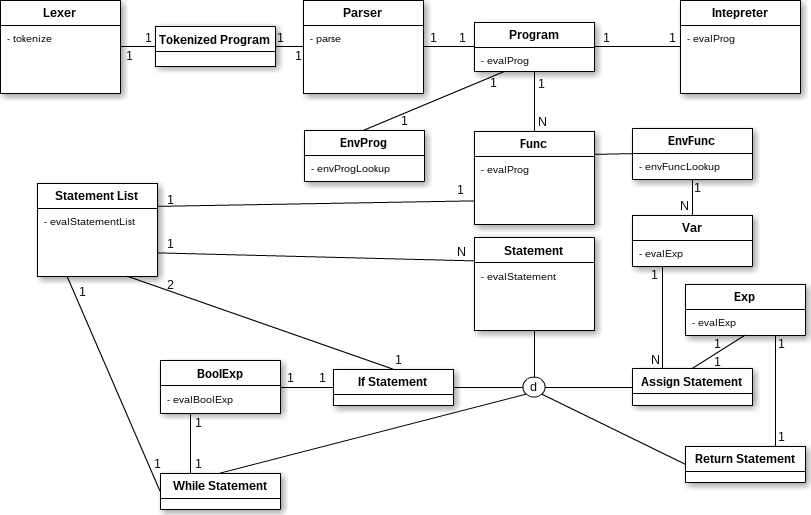
\includegraphics[width=\textwidth]{ClassDiagram.png}
    \caption{Diagrama de clases de la implementaci\'on}
\end{figure}

\begin{figure}[!ht]
    \centering
    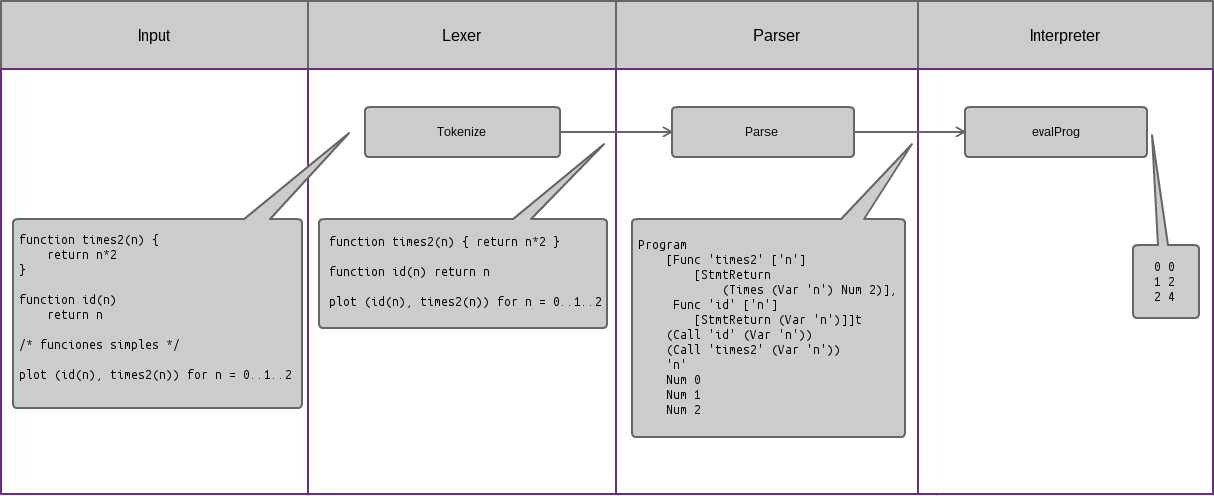
\includegraphics[width=\textwidth]{Flowchart.png}
    \caption{Ejemplo de ejecuci\'on}
\end{figure}


\subsubsection{Modo de uso}
Para compilar el int\'erprete es necesario contar con las aplicaciones 
\textit{Alex}, \textit{Happy} y \textit{ghc} instaladas\footnote{Para esto
puede resultar c\'omodo el programa \textsc{Cabal} que facilita el manejo
de paquetes relacionados con \textsc{Haskell}.}. En la carpeta
\textit{src} incluimos un \textit{Makefile} que genera el ejecutable
\textit{Interprete}.

Para utilizarlo basta con pasarle por \textit{stdin} el c\'odigo a ejecutar.
\begin{verbatim}
cat codigo.cod | ./Interprete
\end{verbatim}
A esto podemos agregarle mediante un \textit{pipe} las instrucci\'on para
\textsc{gnuplot} brindada por la c\'atedra.

\section{Resultados}

\subsection{Gr\'aficos de funciones (ejemplos del ejecuci\'on correcta)}

Para testear el correcto funcionamiento del int\'erprete probamos a plotear las 
funciones provistas por la catedra en los archivos \texttt{hard\_spiral},
\texttt{hard\_mosaico} y \texttt{hard\_koch}. 

Los resultados fueron los siguientes:

\begin{figure}[!ht]
        \centering
        \begin{subfigure}[b]{0.32\textwidth}
                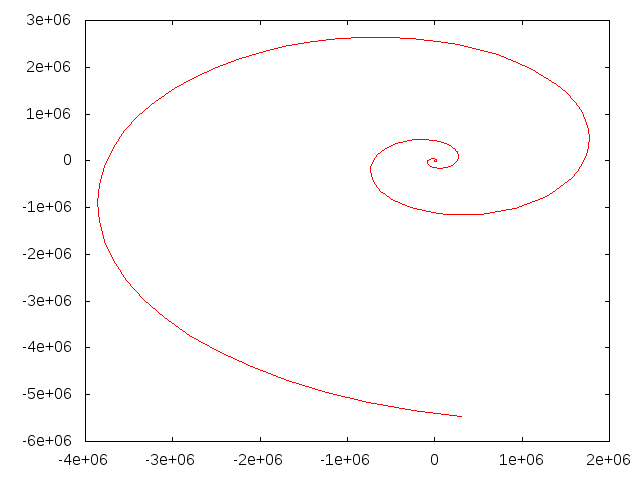
\includegraphics[width=\textwidth]{imgResu/spiral.png}
                \caption{Puntos obtenidos para el archivo \texttt{hard\_spiral}}
        \end{subfigure}%
        ~ %add desired spacing between images, e. g. ~, \quad, \qquad, \hfill etc.
          %(or a blank line to force the subfigure onto a new line)
        \begin{subfigure}[b]{0.32\textwidth}
                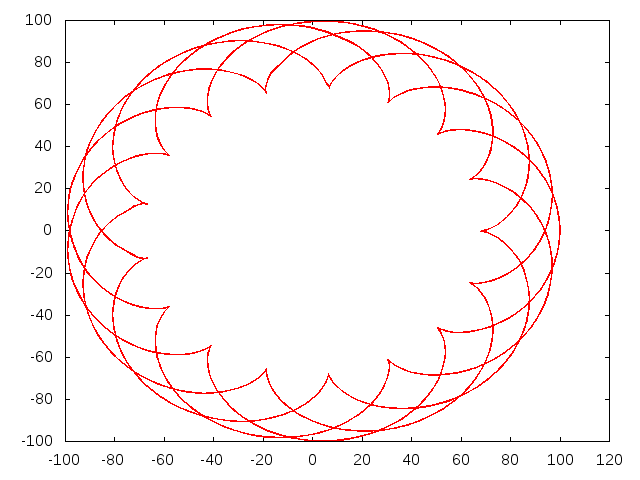
\includegraphics[width=\textwidth]{imgResu/mosaico.png}
                \caption{Puntos obtenidos para el archivo \texttt{hard\_mosaico}}
        \end{subfigure}
        ~ %add desired spacing between images, e. g. ~, \quad, \qquad, \hfill etc.
          %(or a blank line to force the subfigure onto a new line)
        \begin{subfigure}[b]{0.32\textwidth}
                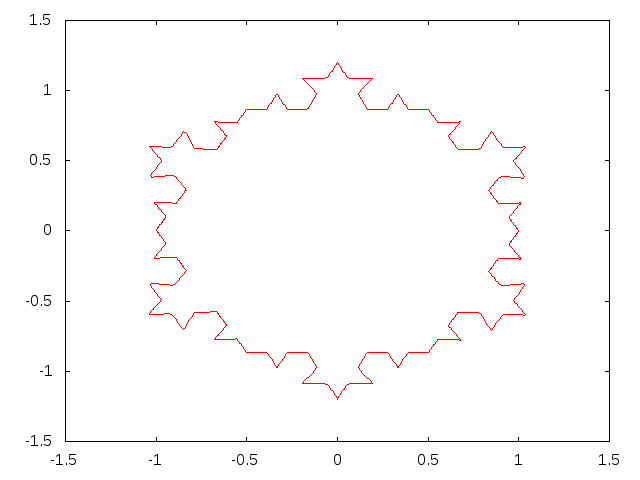
\includegraphics[width=\textwidth]{imgResu/koch.png}
                \caption{Puntos obtenidos para el archivo \texttt{hard\_koch}}
        \end{subfigure}
        \caption{Gr\'aficos obtenidos para las funciones hard: spiral, mosaico y koch}
\end{figure}

M\'as all\'a de que los gr\'aficos parezcan correctos, chequeamos que la diferencia
entre los puntos obtenidos, con los provistos por la c\'atedra, fuera peque\~na.
Vimos que la diferencia rondaba $1{\times}10^{-13}$, con lo cual nos consideramos
satisfechos.

Para realizar este test utilizamos el comando:
\begin{verbatim}
paste archivo1.dat archivo2.dat | awk '{print $3 - $1, $4 - $2}'
\end{verbatim}
que compara, respectivamente, las dos columnas de dos archivos distintos.

\subsubsection{Ambig\"uedades}
La \'unica ambiguedad que encontramos en la especificaci\'on no-formal del
enunciado, es el caso del $if then else$. En particular, en el caso de tener
varios anidados, donde no se use una llave para delimitar el bloque del
\textit{then}. El problema aqu\'i reside en que no es inmediato determinar
a qu\'e \textit{if} corresponde un \textit{else} dado.

Investigando en internet (y recordando un ejercicio de la gu\'ia) llegamos
a la conclusi\'on de que la soluci\'on usual, es la de asociar el \textit{else}
al \textit{if} m\'as cercano (a la izquierda obviamente), como ya fue detallado
previamente.

\subsection{Errores (ejemplos de ejecuci\'on incorrecta)}

Para testear que las herramientas detectaran errores en los archivos 
utilizamos los test brindados por la c\'atedra.

Los resultados en los archivos uno, dos y cinco fueron: 
\subsubsection{Archivo uno}
\begin{verbatim}
Interpreter: 
9:9: Error de parseo. Justo antes de:

(x,10) for x=-1..0.5..5*(pi+(1
\end{verbatim}

\subsubsection{Archivo dos}
\begin{verbatim}
Interpreter: 
4:9: Error de parseo. Justo antes de:

id(x)) for x=-10..0.5..5

/*
\end{verbatim}

\subsubsection{Archivo cinco}
\begin{verbatim}
Interpreter: 
3:14: Error de parseo. Justo antes de:

 {
        return a
    }
\end{verbatim}

Mientras que para el tercer y cuarto archivo fueron:

\subsubsection{Archivo tres}
\begin{verbatim}
Interpreter: 
Runtime error: funcion id no declarada
\end{verbatim}

\subsubsection{Archivo cuatro}
\begin{verbatim}
Interpreter: 
Runtime error: cantidad incorrecta de parametros en constpi
\end{verbatim}

\section{Respuestas a las preguntas del enunciado}

\subsection{Primera pregunta}

Para asegurar est\'aticamente que las guarda del \textit{if} y el
\textit{while} sean booleanos, inducimos a la gram\'atica a s\'olo poder
construir guardas de esa manera. Otros lenguajes de programaci\'on, 
como \textsc{Haskell}, por ejemplo, poseen un sistema de tipado, que les
permite chequear en tiempo de compilaci\'on si los tipos de las expresiones
utilizadas son los correctos.

Un caso distinto es el de \textsc{Python} que no posee tipado est\'atico,
y, m\'as a\'un, muchos objetos puede evaluarse como booleanos.
En este caso el problema puede detectarse \'unicamente en tiempo de
ejecuci\'on.

\subsection{Segunda pregunta}

En el caso de nuestro lenguaje un \texttt{Statement} puede ser una
asignaci\'on, un \textit{if}, un \textit{while} o un \textit{return}.
Los \textit{if} y \textit{while} son `contenedores' de sentencias, con lo cual
podemos analizar el caso asignaci\'on y el caso \textit{return}.

Las asiganciones del lenguaje \textit{MyLanga} hace uso de una variable
del lado izquierdo y una expresi\'on del lado derecho.
Las expresiones son funcionales, en el sentido de que no tienen otro efecto
que devolver un valor. En otros lenguajes (como \textsc{C}), una expresi\'on
puede contener una asignaci\'on (por ejemplo \texttt{a = (b=4);}).
En el caso en que las expresiones puedan contener asignaciones es necesario
un separador expl\'icito, como el punto y coma. Esto se debe a que la secuencia
\begin{verbatim}
a = b
c = 4
\end{verbatim}
puede interpretarse como \texttt{a=(bc=4)} o como
\texttt{a=b ; c=4}.

En nuestro caso las expresiones no pueden contener asignaciones.

\subsection{Tercera pregunta}
En nuestra implementaci\'on no importa el orden en que est\'an definidas las
funciones dentro del c\'odigo. Esto se debe a que primero se parsea todo
el programa, y se genera un \'arbol con las declaraciones de funciones
y el \texttt{plot}. Luego, para ejecutar cada funci\'on, se la busca
y se la ejecuta.
De forma an\'aloga, se soporta recursi\'on, pues nuevamente se busca la
funci\'on que se est\'a ejecutando y se la ejecuta con un contexto
nuevo.

\section{Conclusiones.}
En cuanto a la tecnica map-reduce, nos dimos cuenta que es una herramienta muy útil para realizar consultas que necesiten de agrupamientos o de agregasiones, ya que su forma de funcionar hace que la solución resulte muy intuitiva. Además resulta interesante para realizar procesamiento sobre bases de datos muy voluminosas ya que permite dividir esta en partes y realizar procesos en simultaneo y distribuidos.

El sharding es una herramienta muy útil para balancear la carga de datos entre servidores. MongoDB nos proporciona una forma sencilla de hacerlo, pero que hay que configurar correctamente. La elección de la clave por la que se realizará el sharding (shard key) es muy importante. Esta elección no se puede cambiar una vez se ha establecido.

Los índices son un punto importante a la hora de realizar consultas contra una base de datos MongoDB. Una mala gestión de los índices puede derivar en un rendimiento pobre, por lo que deberemos ser conscientes del tipo de consultas que se realizan a la base de datos. Sabiendo qué campos se utilizan para filtrar y cuáles suelen ser los devueltos en las consultas, seremos capaces de crear los índices necesarios para que nuestra base de datos se comporte correctamente.

Uno de los aspectos que vimos en la sección en la que investigamos sobre Redis y bases de datos key-value, es que al agregar muchas consultas empieza a necesitarse muchos diccionarios (namespaces) perjudicando asi el diseño y aumentando el costo de mantenimiento de la base. Con lo cual el uso de este tipo de bases de datos es mas idoneo para cuando se tienen pocas consultas para las cuales se necesita buena performance.

\include{codigo}


\end{document}
